%===============================================================================
% Artigo SSCAD -- versao condensada da dissertacao de mestrado
% "Investigando Problemas de Escalabilidade de E/S no Algoritmo SDDP em
%  Ambientes HPC" -- Marcelo Barros da Cruz
% Template SBC (single column, 12pt).
%===============================================================================
\documentclass[12pt]{article}

\usepackage{sbc-template}
\usepackage{graphicx,url}
\usepackage[T1]{fontenc}
\usepackage[utf8]{inputenc}
\usepackage{babel}
\babelprovide[import, main]{brazilian}
\usepackage{amsmath,amssymb}
\usepackage{booktabs}
\usepackage{array}
\usepackage{tabularx}
\usepackage{subcaption}

\sloppy

\title{Investigando Problemas de Escalabilidade de E/S no\\ Algoritmo SDDP em Ambientes HPC\thanks{Esse projeto foi parcialmente financiado com recursos de bolsas de produtividade do CNPq (PQ-C: 304308/2025-0) e da FAPERJ (JCNE: E-26/204.481/2025)}}

\author{Marcelo Barros da Cruz\inst{1}, Claudio Luis de Amorim\inst{1}, Diego Leonel Cadette Dutra\inst{1}}

\address{Programa de Engenharia de Sistemas e Computação (PESC) --- COPPE\\ 
Universidade Federal do Rio de Janeiro (UFRJ)\\
Rio de Janeiro --- RJ --- Brasil
  \email{\{mbrcruz, amorim, ddutra\}@cos.ufrj.br}
}

\begin{document}

\maketitle

\begin{abstract}
Efficient I/O scalability remains a major challenge for parallel applications on HPC environments, and is particularly critical in energy-sector optimization models such as Stochastic Dual Dynamic Programming (SDDP), which require frequent, distributed access to large datasets. This paper investigates the I/O bottlenecks of the final simulation phase of SDDP and proposes an MPI-IO architecture over Lustre that replaces the current single-writer strategy. Evaluated on AWS (FSx for Lustre) and the Santos Dumont supercomputer (LNCC), from 2 to 32 nodes, at 32 nodes it reduces total runtime by up to 36.7\% (AWS) and 40.4\% (SDumont), with perceived aggregate bandwidth gains of 113$\times$ and 13.7$\times$, respectively.
\end{abstract}

\begin{resumo}
A escalabilidade eficiente de E/S é um desafio crítico em aplicações paralelas de alto desempenho, sobretudo em modelos de otimização do setor energético como o SDDP, que demandam acesso frequente e distribuído a grandes conjuntos de dados. Este artigo investiga os gargalos de E/S da fase de simulação final do SDDP e propõe uma arquitetura baseada em MPI-IO sobre Lustre, substituindo a estratégia atual com escritor único. Avaliada nos ambientes AWS (FSx for Lustre) e Santos Dumont (LNCC), de 2 a 32 nós, reduz o tempo total em até 36,7\% (AWS) e 40,4\% (SDumont) em 32 nós, com ganhos de banda agregada percebida de 113$\times$ e 13,7$\times$, respectivamente.
\end{resumo}

\section{Introdução}~\label{sec:introducao}

A computação de alto desempenho (\textit{High-Performance Computing} --- HPC) tornou-se ferramenta indispensável para aplicações científicas que processam volumes crescentes de dados~\cite{Kang:20}. Nesses ambientes, o desempenho global de uma aplicação não depende apenas da capacidade computacional dos processadores, mas também da eficiência das operações de entrada e saída (E/S), que frequentemente constituem um dos principais gargalos da execução paralela em larga escala~\cite{Luu:15, Xie:20}. À medida que o número de nós cresce, requisições concorrentes ao sistema de arquivos, contenção sobre adaptadores de rede e custos de coordenação entre processos passam a limitar a escalabilidade efetiva, mesmo quando há paralelismo computacional disponível. Para enfrentar esse desafio, o padrão \textit{Message Passing Interface} (MPI) incorporou, a partir do MPI-2, a especificação MPI-IO, que provê primitivas para acesso paralelo a arquivos compartilhados~\cite{mpi50Cite}. Combinada a sistemas de arquivos paralelos como o Lustre, a MPI-IO permite que múltiplos processos gravem simultaneamente em regiões distintas de um mesmo arquivo, distribuindo a carga de E/S entre vários \textit{Object Storage Targets} (OSTs) e contornando os gargalos típicos de arquiteturas com escritor entralizado~\cite{LustreManual}.

Esse cenário é especialmente relevante para as ferramentas de planejamento da operação de sistemas elétricos. O algoritmo \textit{Stochastic Dual Dynamic Programming} (SDDP)~\cite{MvLm:91} é amplamente usado no despacho hidrotérmico; no Brasil, o Operador Nacional do Sistema Elétrico (ONS) o utiliza no Programa Mensal da Operação (PMO). O algoritmo decompõe o problema em uma malha bidimensional de subproblemas indexados por estágio e cenário; a fase de simulação final --- em que a política já convergida é avaliada em larga escala sobre um conjunto amplo de cenários --- é naturalmente paralela, pois os cenários são mutuamente independentes e podem ser distribuídos entre processos MPI segundo o padrão \textit{bag-of-tasks}~\cite{Cirne:2003}. A transição da operação programada para resolução horária, motivada pela necessidade de capturar horários de ponta, vales e rampas associados à variabilidade das fontes intermitentes, multiplica em uma ordem de grandeza o volume de dados produzido por cenário e estágio~\cite{Ajc:10, Ssr:19}. Nesse regime, a computação deixa de dominar exclusivamente o tempo de execução, que passa a sofrer forte influência das operações de E/S. A arquitetura atual do SDDP concentra todas essas operações em um único processo escritor: cada cenário resolvido envia seu bloco de resultados, via \texttt{MPI\_Send}, ao processo escritor, que serializa as gravações em disco. Essa estratégia introduz dois gargalos: o adaptador de rede do nó escritor, que recebe todas as transferências concorrentes, e o próprio caminho de escrita serializado em um único processo, que não aproveita o paralelismo do sistema de arquivos subjacente. A expansão dos ambientes computacionais utilizados no planejamento energético --- de supercomputadores como o Santos Dumont (LNCC) à nuvem, como a Amazon Web Services (AWS) com FSx for Lustre --- acentua esses gargalos, já que cada plataforma impõe características distintas de hardware, rede e sistema de arquivos.

Este artigo propõe e avalia uma arquitetura paralela de E/S para o SDDP, baseada em escritas independentes com MPI-IO sobre o sistema de arquivos Lustre, com o objetivo de substituir a estratégia atual com processo escritor único. O foco é a \emph{fase de simulação final} do SDDP e, mais especificamente, a \emph{escrita dos resultados} dessa fase, em que se cumula o maior volume de dados. Estão fora do escopo a fase iterativa de geração de cortes, a paralelização das leituras de entrada e o escalonamento de tarefas entre \textit{ranks}, mantido conforme a estratégia \textit{bag-of-tasks} existente. As principais contribuições são: (i) o diagnóstico dos gargalos da arquitetura atual de E/S do SDDP, com identificação do papel do processo escritor único; (ii) a proposta de uma arquitetura de E/S paralela baseada em MPI-IO sobre Lustre, com escritas independentes por processo em \textit{offsets} previamente calculados, preservando o formato dos arquivos consumidos pela cadeia de softwares do planejamento; (iii) a instrumentação detalhada das duas implementações com métricas operacionalmente equivalentes; (iv) a avaliação experimental comparativa em dois ambientes distintos --- AWS com FSx for Lustre dedicado e Santos Dumont com Lustre compartilhado ---, de 2 a 32 nós; e (v) a análise da influência do número de OSTs na escalabilidade da E/S paralela.

O restante deste artigo segue esta organização: a Seção~\ref{sec:fundamentacao} apresenta os conceitos fundamentais, apresentando os detalhes relevantes do SDDP, no contexto deste trabalho; A Seção~\ref{sec:proposta} detalha nossa proposta de melhoria na distribuição de carga de E/S para o SDDP. A Seção~\ref{sec:avaliacoes} traz a avaliação e a análise experimental da abordagem aqui proposta, enquanto a Seção~\ref{sec:relacionados} discute brevemente os principais trabalhos sobre o tema encontrados na literatura. Finalmente, a Seção~\ref{sec:conclusao} fornece as considerações finais e delineia direções para trabalhos futuros. 

\section{Fundamentação}~\label{sec:fundamentacao}

O MPI é o padrão dominante para troca de mensagens (\texttt{MPI\_Send}, \texttt{MPI\_Recv}, operações coletivas) e suporta E/S paralela via MPI-IO a partir do MPI-2~\cite{mpiCite,mpiioCite}. Centralizar resultados em um único escritor transforma a E/S em comunicação ponto a ponto, enquanto o MPI-IO delega a escrita aos processos, deslocando o gargalo para o sistema de arquivos. Em \textit{bag-of-tasks}, o \texttt{MPI\_Send} impõe custo de bloqueio ao remetente que escala com o volume e o número de processos concorrentes por um único receptor. Para E/S paralela, o MPI-IO oferece três abordagens: \emph{escritas independentes} (\texttt{MPI\_File\_write\_at}), simples e robustas para tarefas assíncronas sem exigência de participação coletiva~\cite{Cirne:2003}; \emph{escritas coletivas} (\texttt{MPI\_File\_write\_all}), que sincronizam o comunicador permitindo otimizações por \textit{two-phase I/O} e \textit{data sieving}; e \emph{variantes não bloqueantes} (\texttt{MPI\_File\_iwrite\_at}), que sobrepõem computação e E/S sob a restrição de validade de \textit{buffer}. Complementarmente, o Lustre separa metadados, gerenciados pelo \textit{Metadata Server} (MDS), do fluxo de dados executado com os \textit{Object Storage Servers} (OSSs) e \textit{Object Storage Targets} (OSTs)~\cite{Pjb:02,LustreManual}. O desempenho escala via \textit{striping}, distribuindo blocos (\textit{stripe size}) circularmente por múltiplos OSTs (\textit{stripe count}), onde tamanhos maiores favorecem acessos sequenciais e menores beneficiam concorrência fina.

\subsection{O algoritmo SDDP e sua arquitetura atual de E/S}~\label{sec:sddp}

O SDDP~\cite{MvLm:91} decompõe o planejamento hidrotérmico em subproblemas indexados por $(\text{estágio}, \text{cenário})$, resolvidos em duas fases: na \emph{convergência}, iterações \textit{forward}/\textit{backward} constroem uma política representada por cortes de Benders; na \emph{simulação final}, executada após a convergência, a política fixa é avaliada em larga escala sobre um conjunto amplo de cenários. Este trabalho concentra-se nessa segunda fase, em que os cenários são mutuamente independentes e caracterizam uma aplicação \textit{bag-of-tasks}~\cite{Cirne:2003}: a aplicação particiona os cenários entre os \textit{ranks} MPI e os resolve em paralelo, de modo que o tempo total fica limitado pelo cenário mais lento. É essa natureza que torna a fase escalável, mas também desloca o gargalo da computação para a persistência dos resultados à medida que cresce o número de cenários. A granularidade temporal adotada define o volume produzido: a abordagem tradicional agrega cada estágio em poucos \textit{patamares} de carga, ao passo que a operação moderna requer resolução \emph{horária} --- foco deste trabalho ---, em que cada estágio de um cenário gera dados proporcionais ao número de horas simuladas (p.\,ex.\ 720 registros por par $(\text{estágio}, \text{cenário})$).

Na arquitetura atual (Figura~\ref{fig:arq_atual}), apenas o \textit{rank}~1 (processo escritor) realiza todas as operações de E/S, enquanto o \textit{rank}~0 atua como distribuidor de tarefas. Cada nó, após resolver sua tarefa, envia os resultados por \texttt{MPI\_Send}; o escritor os recebe por \texttt{MPI\_Recv} e grava no sistema de arquivos. Independentemente do número de nós, um único processo concentra a E/S, o que gera dois gargalos: a saturação do adaptador de rede do nó escritor, que recebe todas as transferências concorrentes, e a serialização do fluxo de recepção e escrita. Um atraso do escritor obriga os nós trabalhadores a aguardar, aumentando o custo da execução paralela.

\begin{figure}[ht]
\centering
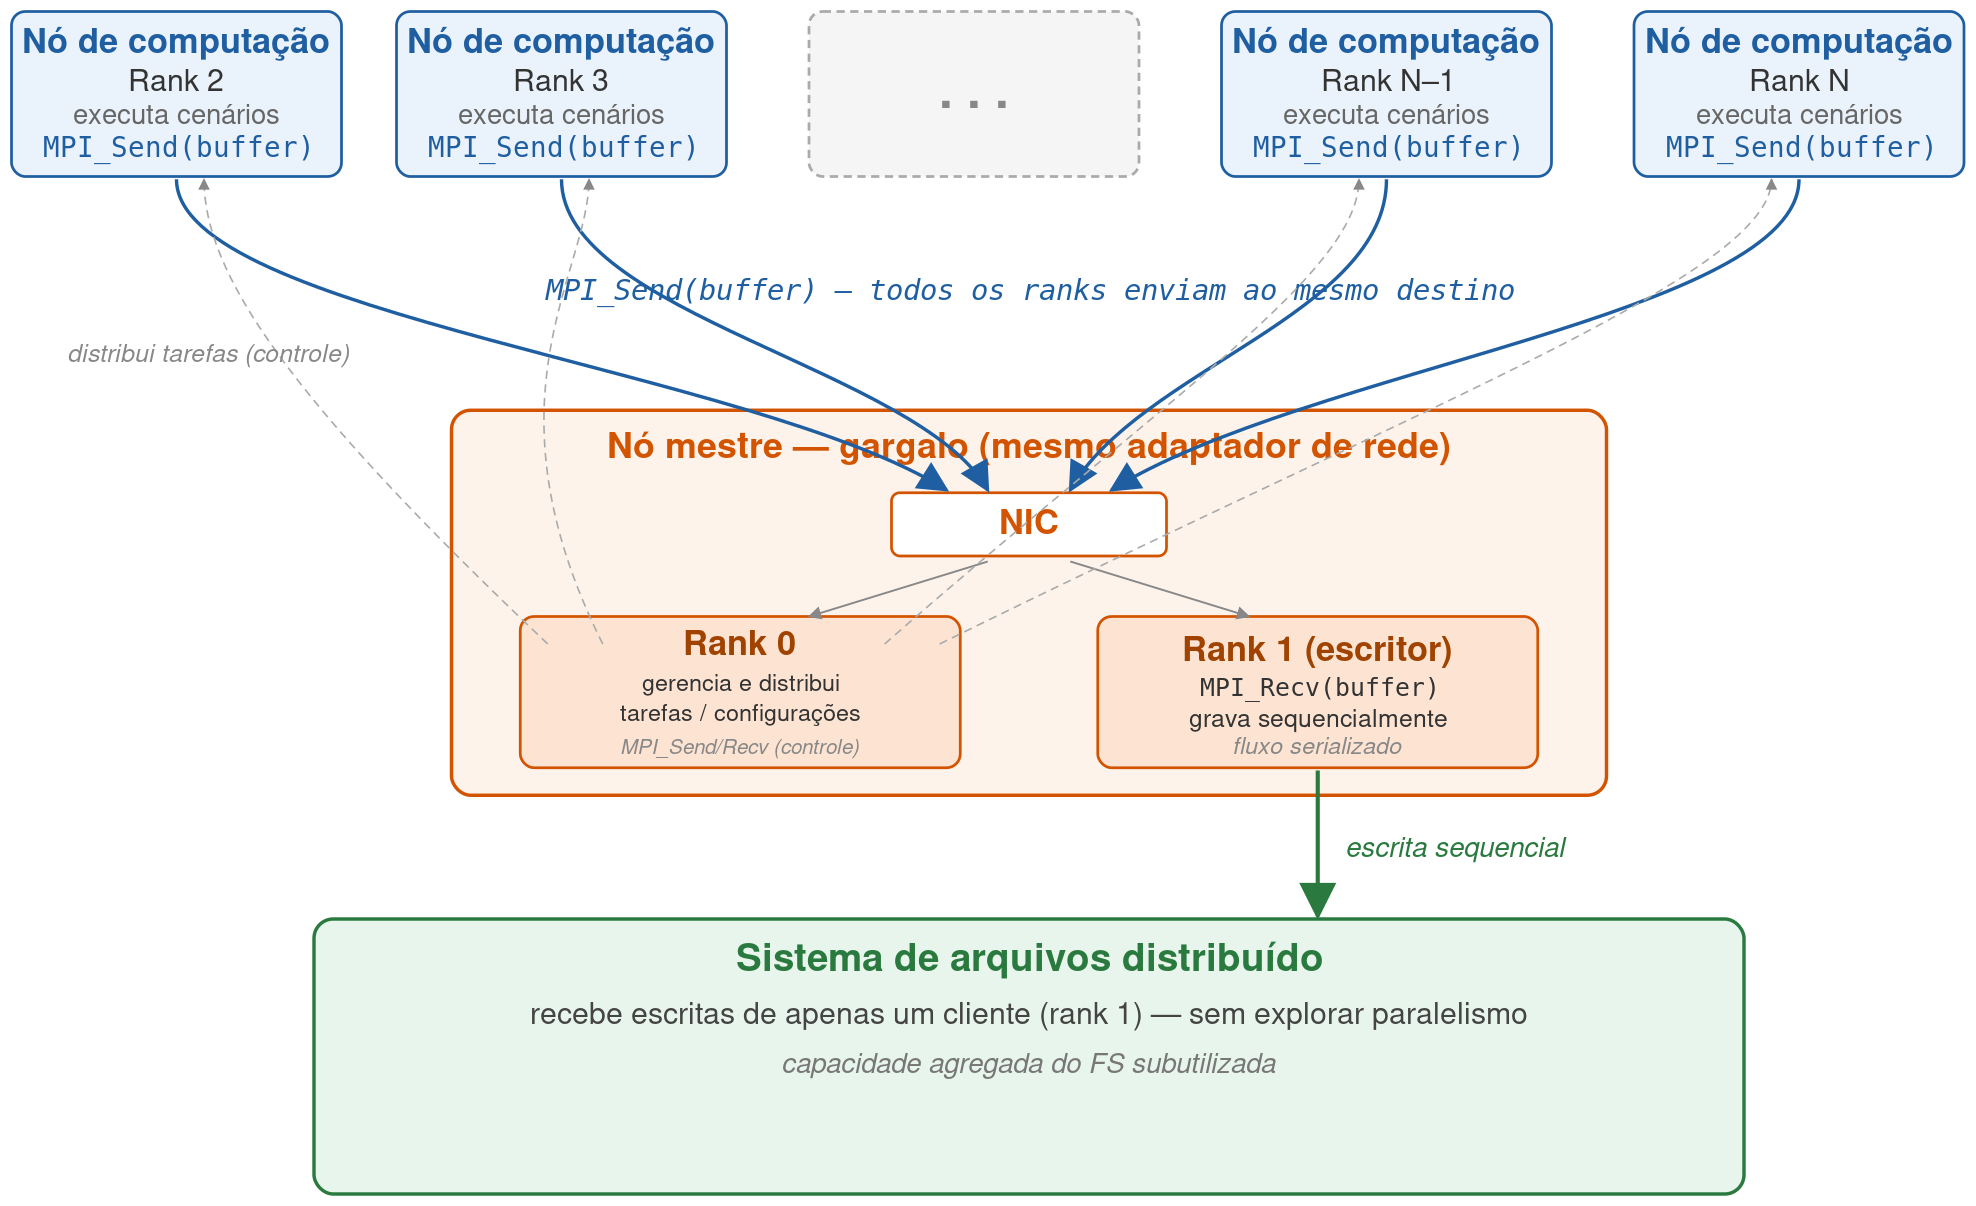
\includegraphics[width=\textwidth]{figuras/SDDP_architecture.png}
\caption{Arquitetura centralizada de E/S do SDDP (implementação atual): o \textit{rank}~0 distribui tarefas, o \textit{rank}~1 é o único escritor e concentra todas as operações de escrita, e os demais \textit{ranks} executam os cenários.}
\label{fig:arq_atual}
\end{figure}

\section{Paralelização dos Mecanismos de E/S do SDDP}~\label{sec:proposta}

Nossa solução substitui o modelo atual por uma organização baseada em MPI-IO sobre o Lustre. Nessa abordagem, cada processo grava diretamente seus próprios resultados em regiões independentes do espaço de saída, evitando a concentração das operações de E/S em um único processo. O ponto central é explorar, simultaneamente, o paralelismo da aplicação MPI e o do sistema de arquivos: como os resultados de diferentes processos são independentes, a aplicação pode posicionar suas escritas previamente e executá-las em paralelo, enquanto o Lustre distribui os arquivos em \textit{stripes} entre diferentes OSTs, atendendo a múltiplas escritas concorrentes e aumentando a banda agregada. A proposta reduz, assim, dois gargalos da arquitetura original: o de comunicação, pois a aplicação deixa de enviar os dados ao processo escritor antes de persistí-los; e o de armazenamento, pois a escrita passa a ser distribuída entre os recursos do sistema de arquivos paralelo em vez de serializada em um único processo. Na arquitetura proposta (Figura~\ref{fig:arq_proposta}), o \textit{rank}~0 segue como distribuidor, enquanto os demais processos gravam seus resultados de forma independente sobre arquivos compartilhados, operando concorrentemente sobre o mesmo arquivo lógico em \textit{offsets} distintos por meio das primitivas do MPI-IO~\cite{mpiioCite}.

\begin{figure}[ht]
\centering

\includegraphics[width=\textwidth]{figuras/SDDP_architecture2.png}
\caption{Arquitetura proposta com MPI-IO e Lustre: o \textit{rank}~0 atua como distribuidor e os demais processos escrevem diretamente em arquivos compartilhados.}
\label{fig:arq_proposta}
\end{figure}

\subsection{Modelo de execução}~\label{sec:modelo_execucao}

A Figura~\ref{fig:timeline} ilustra a linha do tempo da execução segundo a arquitetura proposta, destacando a separação entre o processo distribuidor, a chamada coletiva \texttt{MPI\_File\_open} entre os \textit{ranks}  trabalhadores, as escritas independentes e a chamada \texttt{MPI\_File\_close}. A coordenação global fica restrita aos pontos de abertura e fechamento dos arquivos, enquanto as escritas realizadas após a abertura permanecem independentes. O \textit{rank}~0 distribui as tarefas e, quando não está enviando uma nova tarefa, aguarda o recebimento das concluídas; por isso sua linha é representada integralmente como comunicação. Antes da primeira escrita, os trabalhadores participam de uma abertura coletiva dos arquivos (\texttt{MPI\_File\_open}), que atua como barreira; o distribuidor não participa dessa chamada.

Cada \textit{rank} trabalhador executa o ciclo \textit{bag-of-tasks}: recebe uma tarefa correspondente a um cenário, resolve a simulação e, ao término, efetua escritas independentes nos diversos arquivos de resultado, persistindo os blocos no formato proprietário do SDDP; concluída a persistência, solicita uma nova tarefa. Como o tempo de resolução de cada cenário varia, a distribuição dinâmica conduz a um desbalanceamento natural da carga de escrita entre o trabalhadores. Esse desbalanceamento, intrínseco ao padrão \textit{bag-of-tasks}, dificulta a adoção de escritas coletivas~\cite{Zhang:09CollectiveIO}: chamadas coletivas exigiriam que todos os \textit{ranks} participassem conjuntamente da mesma operação, forçando os processos mais rápidos a aguardar os mais lentos a cada ponto coletivo. Por essas razões, a estratégia de escritas independentes mostra-se mais aderente ao modelo de execução. Quando não há mais cenários a resolver, a aplicação realiza o fechamento coletivo dos arquivos (\texttt{MPI\_File\_close}).

\begin{figure}[ht]
\centering

\includegraphics[width=\textwidth]{figuras/SDDP_timeline_MPIIO.png}
\caption{Linha de tempo da simulação final do SDDP com MPI-IO: os \textit{ranks} trabalhadores executam cenários, sincronizam na abertura coletiva, realizam escritas independentes e sincronizam no fechamento.}
\label{fig:timeline}
\end{figure}

\section{Avaliações}~\label{sec:avaliacoes}

A avaliação compara a implementação atual de E/S com a proposta, focando em tempo de execução, comunicação, largura de banda e bloqueio de E/S~\cite{Rwe:99,Phrrbrw:09} sobre a base PMO/PAR de outubro de 2023. Os experimentos empregaram dois ambientes: a nuvem \textbf{AWS} (com instâncias ENA e Amazon FSx for Lustre sob \textit{Placement Group} \textit{cluster})~\cite{aws:ena, aws:placement} e o supercomputador \textbf{Santos Dumont (SDumont/LNCC)}, com InfiniBand EDR e MPICH 3.2 via \textit{ch3} sobre IP (sem RDMA)~\cite{Fds:03,RlGmmts:05}. 

Para a simulação horária, executaram-se 1.536 cenários com três estágios mensais em ambos os ambientes, com cinco repetições por configuração (reportando média e desvio padrão). O mapeamento utilizou um \textit{rank} por núcleo físico (sem \textit{hyper-threading}), pois o consumo superior a 8~GB de RAM por \textit{rank} esgotaria a capacidade de 384~GB por nó se dobrado. Trata-se de um cenário de \textit{strong scaling}~\cite{Amdahl:67}, com tamanho de problema fixo e variação no número de nós.

A instrumentação via \texttt{MPI\_Wtime} no módulo de persistência assegura comparação direta. A \emph{banda agregada percebida pela aplicação} ($B_w$) expressa a eficiência de E/S para janelas de duração fixa $\Delta$: é a razão entre o volume total gravado e o tempo de E/S do \textit{rank} mais lento da janela ($B_w = \sum V_{i,w} / \max T_{i,w}^{\text{E/S}}$), com valores médios entre janelas e repetições. O uso do processo mais lento no denominador reflete o comportamento síncrono da aplicação ao término de cada janela.

\subsection{Caracterização do \textit{workload} de escrita}

O tamanho dos blocos é determinante para a E/S paralela. Blocos pequenos dominam em \emph{frequência}: 1.801.728 escritas (80,1\% do total) têm até 1~KB, enquanto as faixas intermediárias somam 152.082 (6,8\%), os blocos de até 1~MB respondem por 267.264 (11,9\%) e os de até 50~MB por 27.648 (1,2\%). Em \emph{volume}, porém, o quadro se inverte: praticamente todo o total escrito (cerca de 567~GB) concentra-se nas duas maiores faixas --- aproximadamente 117~GB nos blocos de até 1~MB e 446~GB nos de até 50~MB. Esse contraste --- escritas pequenas predominam em quantidade, grandes em bytes --- decorre da organização dos 117 arquivos de resultado gerados: 104 no formato horário, em que os registros de um par $(\text{estágio}, \text{cenário})$ são acumulados em memória e gravados em uma única operação agregada, e 13 no formato diário, em que cada dia é gravado individualmente, respondendo pela maioria dos blocos pequenos. A alta frequência de operações de granularidade fina tende a aumentar a sobrecarga de metadados, enquanto o volume concentrado nos blocos maiores impõe a maior demanda sobre a largura de banda~\cite{Rwe:99,Phrrbrw:09}.

% =============================================================
\subsection{Experimento AWS}
\label{sec:exp_aws}

O Experimento AWS utilizou 32 nós da instância r7i.12xlarge (Intel Xeon Sapphire Rapids 8488C a 3,2~GHz, 24 núcleos físicos, 384~GB DDR5, rede ENA de até 18,75~Gbps)~\cite{aws:ena}. Empregou-se MPICH~3.2 e um Lustre v2.12 de 12~TB via Amazon FSx, com 1~MDS, 10~OSTs, \textit{stripe count} 10 e \textit{stripes} de 1~MB. Alocou-se um \textit{rank} por núcleo físico, totalizando 24 \textit{ranks} por nó~\cite{intel:23,aws:24}.

Na \textbf{implementação atual} (Tabela~\ref{tab:mpiio_aws}, colunas \emph{atual}), o tempo total cai com o aumento de nós até 16~nós (de 8.971~s em 2~nós para 1.874~s em 16~nós), mas volta a crescer para 2.013~s em 32~nós --- regime saturado típico de \textit{strong scaling} limitado por E/S. A banda degrada-se de 60,5~Gb/s em 2~nós para 3,4~Gb/s em 32~nós, e o percentual do tempo dedicado à E/S cresce de 0,34\% para 49,51\%, coerente com a serialização no nó escritor como ponto de contenção. Na \textbf{implementação MPI-IO} (Tabela~\ref{tab:mpiio_aws}), em que cada processo escreve diretamente no FSx o tempo total decresce monotonicamente até 1.274~s em 32~nós, o tempo de E/S permanece próximo ou abaixo de 1\% a partir de 4~nós e a banda cresce de forma consistente até 380,3~Gb/s em 32~nós.

\begin{table}[ht]
\centering
\caption{Experimento AWS: desempenho das implementações atual e MPI-IO (banda percebida, tempo de E/S, percentual de E/S, tempo de \texttt{MPI\_File\_open}/\texttt{MPI\_File\_close}, tempo total e eficiência). Valores em média\,$\pm$\,desvio padrão de cinco repetições, exceto \% E/S e eficiência (pontuais); eficiência relativa à base de 2~nós; a coluna \emph{open/close} aplica-se apenas à MPI-IO.}
\label{tab:mpiio_aws}
\footnotesize
\setlength{\tabcolsep}{2.5pt}
\renewcommand{\arraystretch}{1.2}
\resizebox{\textwidth}{!}{%
\begin{tabular}{c|ccccc|cccccc}
\toprule
& \multicolumn{5}{c|}{\textbf{Atual}} & \multicolumn{6}{c}{\textbf{MPI-IO}} \\
\textbf{Nós} &
\textbf{\shortstack{Banda\\(Gb/s)}} & \textbf{\shortstack{E/S\\(s)}} & \textbf{\% E/S} & \textbf{\shortstack{Total\\(s)}} & \textbf{Efic.} &
\textbf{\shortstack{Banda\\(Gb/s)}} & \textbf{\shortstack{E/S\\(s)}} & \textbf{\% E/S} & \textbf{\shortstack{\emph{open}/\\\emph{close} (s)}} & \textbf{\shortstack{Total\\(s)}} & \textbf{Efic.} \\
\midrule
2  & $60{,}5{\pm}5{,}2$  & $30{,}9{\pm}13{,}2$ & $0{,}3\%$  & $8\,971{\pm}349$ & $100\%$ & $57{,}0{\pm}8{,}5$   & $19{,}0{\pm}5{,}6$ & $0{,}2\%$ & $42{,}5{\pm}7{,}7$   & $8\,859{\pm}111$ & $100\%$ \\
4  & $51{,}3{\pm}2{,}8$  & $78{,}2{\pm}27{,}8$ & $1{,}6\%$  & $4\,823{\pm}53$  & $93\%$  & $106{,}0{\pm}19{,}4$ & $12{,}8{\pm}3{,}5$ & $0{,}3\%$ & $51{,}2{\pm}15{,}2$  & $5\,127{\pm}108$ & $86\%$ \\
8  & $18{,}9{\pm}3{,}8$  & $201{,}7{\pm}53{,}3$ & $7{,}6\%$  & $2\,639{\pm}18$  & $85\%$  & $167{,}0{\pm}40{,}2$ & $10{,}8{\pm}6{,}3$ & $0{,}4\%$ & $69{,}8{\pm}4{,}7$   & $2\,600{\pm}37$  & $85\%$ \\
16 & $4{,}5{\pm}0{,}3$   & $527{,}9{\pm}53{,}1$ & $28{,}2\%$ & $1\,874{\pm}57$  & $60\%$  & $274{,}2{\pm}15{,}3$ & $7{,}5{\pm}1{,}8$  & $0{,}5\%$ & $83{,}5{\pm}4{,}2$   & $1\,558{\pm}9$   & $71\%$ \\
32 & $3{,}4{\pm}0{,}1$   & $996{,}6{\pm}167{,}0$ & $49{,}5\%$ & $2\,013{\pm}29$  & $28\%$  & $380{,}3{\pm}30{,}7$ & $9{,}0{\pm}2{,}5$  & $0{,}7\%$ & $147{,}3{\pm}7{,}3$  & $1\,274{\pm}24$  & $44\%$ \\
\bottomrule
\end{tabular}
}
\end{table}

A comparação direta (Tabela~\ref{tab:comparativo_aws}) evidencia o ganho: a melhoria no tempo total é pequena em 2~nós, torna-se negativa em 4~nós, mas passa a positiva a partir de 8~nós, crescendo até 36,7\% em 32~nós. A banda MPI-IO passa de ligeiramente inferior em 2~nós para 2,07$\times$ em 4~nós, 8,82$\times$ em 8~nós, 60,66$\times$ em 16~nós e 113,00$\times$ em 32~nós, e a redução do tempo de E/S chega a 99,1\% em 32~nós.

\begin{table}[ht]
\centering
\caption{Experimento AWS: resumo comparativo atual $\times$ MPI-IO (melhorias calculadas em relação à implementação atual; valores negativos indicam piora).}
\label{tab:comparativo_aws}
\footnotesize
\setlength{\tabcolsep}{5pt}
\renewcommand{\arraystretch}{1.15}
\begin{tabular}{ccccccc}
\toprule
\textbf{Nós} & \textbf{\shortstack{Total\\atual (s)}} & \textbf{\shortstack{Total\\MPI-IO (s)}} &
\textbf{\shortstack{Melhoria\\total}} & \textbf{\shortstack{Ganho de\\banda}} &
\textbf{\shortstack{E/S atual\\(s)}} & \textbf{\shortstack{Melhoria\\E/S}} \\
\midrule
2  & $8\,971$ & $8\,859$ & $1{,}3\%$   & $0{,}94\times$   & $30{,}9$  & $38{,}5\%$ \\
4  & $4\,823$ & $5\,127$ & $-6{,}3\%$  & $2{,}07\times$   & $78{,}2$  & $83{,}7\%$ \\
8  & $2\,639$ & $2\,600$ & $1{,}5\%$   & $8{,}82\times$   & $201{,}7$ & $94{,}7\%$ \\
16 & $1\,874$ & $1\,558$ & $16{,}8\%$  & $60{,}66\times$  & $527{,}9$ & $98{,}6\%$ \\
32 & $2\,013$ & $1\,274$ & $36{,}7\%$  & $113{,}00\times$ & $996{,}6$ & $99{,}1\%$ \\
\bottomrule
\end{tabular}
\end{table}

A Figura~\ref{fig:banda_aws} apresenta a banda agregada percebida, com curvas qualitativamente opostas. A implementação atual parte de 60,5~Gb/s em 2~nós --- em pequena escala chega a superar a MPI-IO (57,0~Gb/s), pois o gargalo do escritor único ainda não saturou e o custo fixo da coordenação pesa relativamente --- mas degrada-se mais de uma ordem de grandeza (18,9~Gb/s em 8~nós; 4,5 em 16; 3,4 em 32) à medida que a serialização no nó escritor se torna o ponto de contenção. A MPI-IO, ao contrário, cresce monotonicamente (106,0~Gb/s em 4~nós; 167,0 em 8; 274,2 em 16; 380,3 em 32), pois distribui as escritas entre os processos e os múltiplos OSTs do FSx --- um ganho sobre a implementação atual que passa de 2,07$\times$ em 4~nós a 8,82$\times$ em 8, 60,66$\times$ em 16 e 113,00$\times$ em 32~nós.

A Figura~\ref{fig:tempo_aws} decompõe o tempo de execução. Na implementação atual, a fração de E/S cresce de 7,6\% em 8~nós para 28,2\% em 16 e 49,5\% em 32, fazendo o tempo total saturar em 16~nós e \emph{piorar} em 32~nós (de 1.874 para 2.013~s): acrescentar nós deixa de compensar. Na MPI-IO, a E/S permanece abaixo de 1\% a partir de 4~nós e o tempo total decresce monotonicamente até 1.274~s em 32~nós, o que corresponde a reduções de 1,5\%, 16,8\% e 36,7\% em 8, 16 e 32~nós. A única parcela que cresce em termos relativos na MPI-IO é a das chamadas \texttt{MPI\_File\_open}/\texttt{MPI\_File\_close} (coluna \emph{open/close} da Tabela~\ref{tab:mpiio_aws}), de 42,5~s (0,5\%) em 2~nós a 147,3~s (11,6\%) em 32. Esse custo é pago uma única vez por execução, na abertura e no fechamento dos arquivos (início e fim), e \emph{independe do tamanho da carga}: não cresce com o número de cenários nem de estágios, dependendo apenas do número de nós que participam da operação coletiva. Por isso sua fração percentual aparece inflada, já que estes experimentos usam apenas três estágios mensais; mantido o mesmo número de nós, ao quadruplicar o horizonte (de 3 para 12 estágios) todas as componentes da decomposição crescem proporcionalmente enquanto esse custo permanece inalterado, tornando-se desprezível frente ao tempo total.

\begin{figure}[ht]
\centering
\begin{subfigure}[b]{0.49\textwidth}
\centering
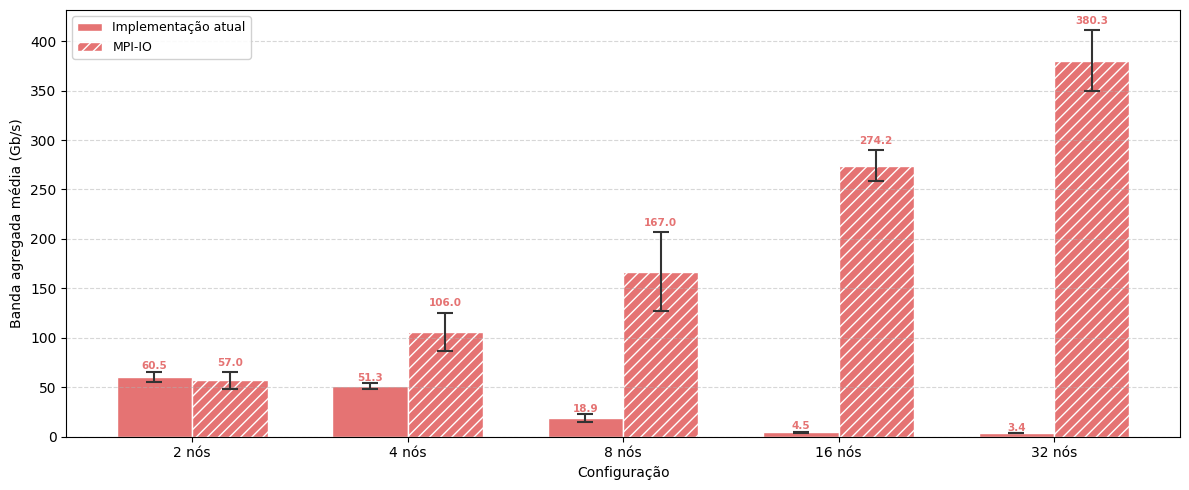
\includegraphics[width=\textwidth]{figuras/Banda_AWS.png}
\caption{Banda agregada percebida.}
\label{fig:banda_aws}
\end{subfigure}\hfill
\begin{subfigure}[b]{0.49\textwidth}
\centering

\includegraphics[width=\textwidth]{figuras/Tempo_execucao_AWS.png}
\caption{Tempo de execução.}
\label{fig:tempo_aws}
\end{subfigure}
\caption{Experimento AWS: (a) banda agregada percebida e (b) tempo de execução.}
\label{fig:aws}
\end{figure}

\subsubsection{Impacto do número de OSTs}~\label{sec:osts}

Para isolar o efeito da infraestrutura de armazenamento, comparou-se, na abordagem MPI-IO, configurações de 4 e 10~OSTs em 16 e 32~nós, mantidos constantes os demais parâmetros. A Figura~\ref{fig:osts_banda} mostra que, em 16~nós, 10~OSTs atingem 274,2~Gb/s contra 49,4~Gb/s com 4~OSTs (ganho de 5,6$\times$). Ao passar para 32~nós, as tendências se opõem: com 10~OSTs a banda cresce para 380,3~Gb/s, enquanto com 4~OSTs cai para 16,1~Gb/s --- ganho de 23,6$\times$. O tempo médio de envio nas classes de maior volume também se reduz drasticamente com mais OSTs (p.\,ex.\ de 309~ms para 13,8~ms nas mensagens de até 1~MB em 32~nós). Quando a concorrência entre processos aumenta, a configuração com menos OSTs limita a escalabilidade da E/S, indicando que o dimensionamento da camada de armazenamento deve ser tratado como parâmetro de projeto.

\begin{figure}[ht]
\centering

\includegraphics[width=.62\textwidth]{figuras/Experimento_OSTs_banda.png}
\caption{Banda agregada percebida na implementação MPI-IO para 4 e 10~OSTs em
16 e 32~nós (Experimento AWS).}
\label{fig:osts_banda}
\end{figure}

% =============================================================
\subsection{Experimento SDumont}
\label{sec:exp_sdumont}

O Experimento SDumont utilizou até 32~nós (dois Intel Xeon Cascade Lake Gold 6252, 24 núcleos físicos, 384~GB, InfiniBand EDR de 100~Gb/s), MPICH~3.2 e um Lustre v2.12 (ClusterStor L300 da Cray/HPE) com 1~MDS e 6~OSTs, \textit{stripe count} 6 e \textit{stripes} de 1~MB. Diferentemente do FSx dedicado da AWS, o sistema de arquivos do SDumont é \emph{compartilhado} com outras cargas de HPC, o que introduz variabilidade e amplifica a contenção nas maiores escalas --- cenário mais desafiador para a escalabilidade de E/S.

O padrão observado na AWS se repete (Tabela~\ref{tab:mpiio_sdumont}). Na implementação atual, o tempo total decresce até 16~nós (3.130~s), mas piora em 32~nós (3.744~s), e a banda colapsa de 27,9~Gb/s em 2~nós para 2,5~Gb/s em 32~nós, com a parcela de E/S saltando para 45,83\%. Na MPI-IO, o tempo total decresce em toda a faixa (até 2.233~s em 32~nós), a banda cresce consistentemente até 34,1~Gb/s e a E/S permanece abaixo de 5\% em todas as configurações. A comparação direta mostra sobrecusto em pequena escala (--1,9\% em 2~nós), mas ganhos crescentes a partir de 8~nós: 19,5\% em 16~nós e 40,4\% em 32~nós, com ganho de banda de 4,50$\times$ e 13,70$\times$ e redução do tempo de E/S de 87,3\% e 96,3\%, respectivamente.

\begin{table}[ht]
\centering
\caption{Experimento SDumont: desempenho das implementações atual e MPI-IO (banda percebida, tempo de E/S, tempo de \texttt{MPI\_File\_open}/\texttt{MPI\_File\_close}, tempo total e eficiência). Valores em média\,$\pm$\,desvio padrão de cinco repetições, exceto eficiência (pontual); eficiência relativa à base de 2~nós; a coluna \emph{open/close} aplica-se apenas à MPI-IO.}
\label{tab:mpiio_sdumont}
\footnotesize
\setlength{\tabcolsep}{2.5pt}
\renewcommand{\arraystretch}{1.2}
\resizebox{\textwidth}{!}{%
\begin{tabular}{c|cccc|ccccc}
\toprule
& \multicolumn{4}{c|}{\textbf{Atual}} & \multicolumn{5}{c}{\textbf{MPI-IO}} \\
\textbf{Nós} &
\textbf{\shortstack{Banda\\(Gb/s)}} & \textbf{\shortstack{E/S\\(s)}} & \textbf{\shortstack{Total\\(s)}} & \textbf{Efic.} &
\textbf{\shortstack{Banda\\(Gb/s)}} & \textbf{\shortstack{E/S\\(s)}} & \textbf{\shortstack{\emph{open}/\\\emph{close} (s)}} & \textbf{\shortstack{Total\\(s)}} & \textbf{Efic.} \\
\midrule
2  & $27{,}9{\pm}7{,}1$ & $79{,}3{\pm}32{,}8$   & $14\,524{\pm}24$ & $100\%$ & $5{,}5{\pm}0{,}4$  & $321{,}2{\pm}85{,}2$ & $23{,}2{\pm}3{,}0$   & $14\,796{\pm}46$  & $100\%$ \\
4  & $24{,}8{\pm}6{,}7$ & $123{,}2{\pm}49{,}5$  & $7\,758{\pm}28$  & $94\%$  & $8{,}9{\pm}1{,}0$  & $271{,}5{\pm}50{,}0$ & $32{,}3{\pm}1{,}6$   & $7\,800{\pm}93$   & $95\%$ \\
8  & $23{,}9{\pm}4{,}8$ & $210{,}9{\pm}79{,}4$  & $4\,265{\pm}63$  & $85\%$  & $12{,}1{\pm}1{,}5$ & $194{,}7{\pm}34{,}4$ & $79{,}3{\pm}21{,}9$  & $4\,251{\pm}142$  & $87\%$ \\
16 & $4{,}2{\pm}0{,}3$  & $795{,}7{\pm}87{,}7$  & $3\,130{\pm}73$  & $58\%$  & $18{,}9{\pm}1{,}2$ & $100{,}9{\pm}21{,}1$ & $126{,}5{\pm}28{,}3$ & $2\,519{\pm}101$  & $73\%$ \\
32 & $2{,}5{\pm}0{,}5$  & $1\,715{,}8{\pm}259{,}8$ & $3\,744{\pm}249$ & $24\%$  & $34{,}1{\pm}5{,}4$ & $64{,}1{\pm}27{,}0$  & $230{,}0{\pm}8{,}9$  & $2\,233{\pm}87$   & $41\%$ \\
\bottomrule
\end{tabular}
}
\end{table}

A Figura~\ref{fig:banda_sdumont} confirma o contraste de \emph{comportamento}: a implementação atual preserva banda elevada até 8~nós, mas colapsa a partir de 16~nós (entre 2,5 e 4,2~Gb/s), enquanto a MPI-IO cresce monotonicamente até 34,1~Gb/s em 32~nós. Diferentemente da AWS, porém, o SDumont é um supercomputador \emph{compartilhado} em que centenas de \textit{jobs} de diferentes usuários disputam simultaneamente os mesmos servidores de metadados e OSTs do Lustre. Essa concorrência externa impõe um teto de banda que atinge toda a aplicação: mesmo com a solução MPI-IO, a banda máxima no SDumont (34,1~Gb/s) fica cerca de uma ordem de grandeza \emph{abaixo} da obtida na AWS com FSx dedicado (380,3~Gb/s). A escrita paralela preserva, portanto, a vantagem estrutural em relação ao escritor único. A Figura~\ref{fig:tempo_sdumont} decompõe o tempo médio por processo: na implementação atual, a parcela de E/S cresce marcadamente a partir de 16~nós, enquanto na MPI-IO ela permanece reduzida e o custo de \texttt{MPI\_File\_open}/\texttt{MPI\_File\_close} (coluna \emph{open/close} da Tabela~\ref{tab:mpiio_sdumont}, de 23,2~s a 230,0~s de 2 a 32~nós) compõe a fração visível nas maiores configurações --- pelo mesmo motivo já discutido para a AWS: um custo pago uma única vez, independente da carga e apenas inflado pelo horizonte reduzido destes experimentos. A queda de eficiência em 32~nós (24,2\% na atual e 41,4\% na MPI-IO) e a variabilidade refletem o caráter compartilhado do Lustre do SDumont; ainda assim, a vantagem estrutural da escrita paralela persiste em toda a faixa.

\begin{figure}[ht]
\centering
\begin{subfigure}[b]{0.49\textwidth}
\centering

\includegraphics[width=\textwidth]{figuras/Banda_SDumont.png}
\caption{Banda agregada percebida.}
\label{fig:banda_sdumont}
\end{subfigure}\hfill
\begin{subfigure}[b]{0.49\textwidth}
\centering

\includegraphics[width=\textwidth]{figuras/Tempo_execucao_SDumont.png}
\caption{Decomposição do tempo médio por processo.}
\label{fig:tempo_sdumont}
\end{subfigure}
\caption{Experimento SDumont: (a) banda agregada percebida e (b) decomposição do tempo médio por processo.}
\label{fig:sdumont}
\end{figure}

\subsection{Síntese das avaliações}~\label{sec:sintese}

Os dois experimentos convergem para um diagnóstico comum, ainda que com magnitudes diferentes. Em pequena escala (2 e 4~nós), a implementação atual é competitiva ou ligeiramente superior, pois o gargalo do escritor único ainda não saturou e o custo fixo da camada MPI-IO pesa relativamente. Nas maiores escalas, o quadro se inverte --- na AWS a partir de 8~nós, no SDumont a partir de 16~nós ---, com a degradação da implementação atual refletindo a contenção sobre a serialização no nó escritor, enquanto a MPI-IO exibe perfil monotonicamente crescente de banda. Esse contraste qualitativo de comportamento --- e não apenas o ganho pontual em uma escala --- é o resultado mais robusto. A magnitude do benefício, porém, depende fortemente da infraestrutura: no FSx dedicado da AWS, a proposta atinge 380,3~Gb/s em 32~nós (113$\times$ sobre a atual) e reduz o tempo total em até 36,7\%; no Lustre compartilhado do SDumont, chega a 34,1~Gb/s (13,7$\times$) e reduz o tempo total em até 40,4\%, mesmo sob concorrência com outras cargas. A preservação da vantagem estrutural nesse regime sugere que a arquitetura é portátil entre ambientes heterogêneos.

\section{Trabalhos relacionados}~\label{sec:relacionados}

Dickens e Logan~\cite{Dickens:08} introduziram o uso de MPI-IO sobre Lustre, mostrando que, para padrões não-\textit{interleaved} --- em que cada processo escreve em região exclusiva ---, escritas independentes evitam a contenção de \textit{locks} e superam as coletivas; esse diagnóstico fundamenta a escolha de \texttt{MPI\_File\_write\_at} neste trabalho. Gropp \textit{et al.}~\cite{Gropp:08} formalizaram que, nesse regime, \texttt{MPI\_File\_write\_all} degenera para uma escrita simples acrescida de sincronização, tornando as coletivas estritamente piores --- exatamente o padrão de acesso do SDDP. Liao \textit{et al.}~\cite{LiaoIPDPS:07} demonstraram que escritas menores que uma unidade de \textit{stripe} forçam múltiplos \textit{locks} sequenciais e propuseram \textit{two-stage write-behind buffering} alinhado às fronteiras de \textit{stripe}; este trabalho não adota alinhamento explícito, mas parte das escritas do SDDP horário alinha-se incidentalmente ao \textit{stripe} de 1~MB, o que ajuda a explicar o desempenho obtido. Dickens e Thakur~\cite{Dickens:10} e Liao e Choudhary~\cite{Liao:08} exploram estratégias adicionais de alinhamento e particionamento adaptativo para reduzir contenção no Lustre. Por fim, García-Carballeira \textit{et al.}~\cite{GarciaCarballeiraISPDC:23} apresentam o \emph{Expand Ad-Hoc}, um sistema de arquivos efêmero em espaço de usuário sobre o armazenamento local dos nós; compor a proposta com uma camada desse tipo poderia contornar a contenção externa observada no SDumont, com migração ao Lustre apenas no \textit{stage-out}.

\section{Conclusões}~\label{sec:conclusao}

Este trabalho diagnosticou e resolveu o gargalo crítico de E/S na fase de simulação final do algoritmo SDDP, substituindo a arquitetura legada de um único processo escritor por uma abordagem paralela baseada em escritas independentes com MPI-IO no sistema de arquivos Lustre. A avaliação experimental conduzida em dois ambientes distintos — um sistema em nuvem com armazenamento dedicado (AWS/FSx) e um supercomputador tradicional com recursos compartilhados (LNCC/Santos Dumont) — evidenciou que a solução proposta elimina a contenção de rede e a serialização no nó mestre, garantindo escalabilidade em larga escala.

Mais do que os ganhos expressivos de desempenho e largura de banda observados em 32 nós, o resultado mais robusto deste estudo é o contraste qualitativo de comportamento: enquanto a estratégia centralizada colapsa devido à saturação do escritor, a arquitetura com MPI-IO exibe um perfil de escalabilidade monotonicamente crescente em ambas as infraestruturas. Isso demonstra não apenas a eficácia técnica da abordagem, mas também a sua portabilidade entre ecossistemas heterogêneos de computação de alto desempenho. Ademais, a análise do impacto do número de OSTs reforça que o dimensionamento da camada de armazenamento (stripe count e stripe size) não deve ser tratado como um detalhe acessório, mas sim como um parâmetro estrutural de projeto em aplicações data-intensive.

Como direções para trabalhos futuros, destacam-se a reestruturação do modelo de persistência dos arquivos diários para mitigar o overhead de E/S granular; a exploração de interconexões de altíssima velocidade, como InfiniBand HDR/NDR e AWS EFA, combinada a políticas de bufferização estritamente alinhadas às fronteiras de stripe do Lustre; a reavaliação de escritas coletivas com \textit{two-phase I/O} mediante o redesenho da sincronização de chamadas; e, por fim, a extensão dessa arquitetura paralela para a fase iterativa de geração de cortes do SDDP.


\bibliographystyle{sbc}
\bibliography{bibliografy}

\end{document}
